\documentclass[
    hyperref={bookmarks=false,colorlinks=true, linkcolor=blue, urlcolor=blue, citecolor=MidnightBlue},
    xcolor={dvipsnames},
]{beamer}

\usetheme[height=8mm]{Rochester}
\usecolortheme{default}

% \usepackage{pgfpages} % For viewing slides on the right
\usepackage[warningthreshold=0.95]{resizegather} % For resizing gather environment to fit massive equations
\setbeameroption{show notes} % Shows notes on the right of the main slides
% \setbeameroption{show notes on second screen}
\usefonttheme[onlymath]{serif} % For serif font in math mode
\usepackage[round]{natbib} % Needed for Author name citations
\usepackage{../../packages/shared}
\usepackage{../../packages/misc_commands}
% =========================
% Causal Structure Diagrams
% =========================
\definecolor{obs_outline}{RGB}{51,157,215}
\definecolor{obs_fill}{RGB}{222,253,255}
\definecolor{obs_text}{RGB}{0,0,0}
\definecolor{lat_outline}{RGB}{251,141,54}
\definecolor{cause}{RGB}{30, 0, 30}
\definecolor{lat_fill}{RGB}{255,213,153}
\definecolor{lat_text}{RGB}{0,0,0}
\tikzset{square/.style={regular polygon,regular polygon sides=4}}
\tikzset{triangle/.style={regular polygon,regular polygon sides=3}}
\tikzset{observed/.style={obs_text, align=center, triangle, thick, draw=obs_outline, fill=obs_fill, inner sep=-0.2em, text width=1.5em}}
\tikzset{latent/.style={lat_text, align=center, circle, thick, draw=lat_outline, fill=lat_fill, text width=1.5em, inner sep=0.2em}}
\tikzset{fade/.style={opacity=0.2}}
\tikzset{unfade/.style={opacity=1.0}}
% TikZ stile to apply keys only on specific beamer overlays
% onslide=<overlay spec>{key=value, key=value, ...}
\tikzset{onslide/.code args={<#1>#2}{%
  \only<#1>{\pgfkeysalso{#2}}%
}}
\providecommand{\p}[1]{#1}
% \tikzset{cause/.style={mid arrow/.style={postaction={decorate,decoration={markings, mark=at position .5 with {\arrow[#1]{stealth}}}}},}}
\tikzset{
    % style to apply some styles to each segment of a path
    on each segment/.style={
        decorate,
        decoration={
            show path construction,
            moveto code={},
            lineto code={
                \path [#1]
                (\tikzinputsegmentfirst) -- (\tikzinputsegmentlast);
            },
            curveto code={
                \path [#1] (\tikzinputsegmentfirst)
                .. controls
                (\tikzinputsegmentsupporta) and (\tikzinputsegmentsupportb)
                ..
                (\tikzinputsegmentlast);
            },
            closepath code={
                \path [#1]
                (\tikzinputsegmentfirst) -- (\tikzinputsegmentlast);
            },
        },
    },
    % style to add an arrow in the middle of a path
    mid arrow/.style={postaction={decorate,decoration={
                markings,
                mark=at position .6 with {\arrow[scale=1.5, cause]{stealth}}
            }}},
}
% =========================
% ========================= % Causal structure formatting for tikz
\renewcommand{\term}[1]{\textcolor{Mahogany}{#1}}
\renewcommand{\tcdot}{\cdot} % Tentative cdot, not sure if I want to keep dots


\title[Triangle Inequalities]{Causal Compatibility Inequalities Admitting of Quantum Violations in the Triangle Scenario}
\author[Fraser]{T.C.~Fraser\inst{1,2}}
\institute
{
    \inst{1}%
    Perimeter Institute for Theoretical Physics\\
    Ontario, Canada \\
    \inst{2}%
    University of Waterloo\\
    Ontario, Canada \\
}
\date[QN 2016]{Quantum Networks Workshop, IIP, Nov. 2016}

\begin{document}

\frame{\titlepage}

\begin{frame}[allowframebreaks]
    \frametitle{References}
    \todo[TC]{Figure out how to get references at the end}
    \setbeamertemplate{bibliography item}{\insertbiblabel}
    \bibliographystyle{plainnat}
    \bibliography{../references}{}
\end{frame}

% \begin{frame}
%     \frametitle{Table of Contents}
% \tableofcontents

% \end{frame}


\begin{frame}
    \frametitle{Introduction}
    \note[item]{Thank International Institute for Physics (IIP) for support}
    \note[item]{Thank Perimeter Institute for Theoretical Physics (PI) for support}
\end{frame}
\begin{frame}
    \frametitle{Objective}
    \begin{itemize}
        \item Derive causal compatibility/locality inequalities that distinguish quantum distributions from classical ones
        \item Specifically for the Triangle Scenario (TS)
    \end{itemize}
    \begin{center}
        \scalebox{1.0}{\begin{tikzpicture}[scale=1]
    \begin{scope}[every node/.style=observed]
        \node (C) at (-2, 0) {$C$};
        \node (B) at (2, 0) {$B$};
        \node (A) at (0, {2*sqrt(3)}) {$A$};
    \end{scope}
    \begin{scope}[every node/.style=latent]
        \node (X) at (-1, {sqrt(3)}) {$X$};
        \node (Y) at (1, {sqrt(3)}) {$Y$};
        \node (Z) at (0, 0) {$Z$};
    \end{scope}
    \begin{scope}[every path/.style={draw=cause, thick}]
        \path[postaction={on each segment={mid arrow}}]
        (X) -- (A)
        (X) -- (C)
        (Y) -- (A)
        (Y) -- (B)
        (Z) -- (B)
        (Z) -- (C);
    \end{scope}
\end{tikzpicture}}
    \end{center}
    \note[item]{Research project's goal was to derive new causal compatibility inequalities that distinguish quantum correlations from classical correlations}
    \note[item]{More specifically, the ambition of the project is to obtain such inequalities that constraint compatibility with The Triangle Scenario}
    \note[item]{Triangle Scenario has be studied extensively before}
\end{frame}

\begin{frame}
    \frametitle{Objective Cont'd}
    \begin{itemize}
        \item In~\citet{Branciard_2012} it was noted that characterizing locality in TS remained an open problem and that identifying compatibility constraints in this configuration \textbf{seemed challenging}
        \item In~\citet{Fritz_2012}, Fritz demonstrated that TS is the \textbf{smallest} correlation scenario in which their exists quantum incompatible distributions (proof without inequalities)
        \item In~\citet{Henson_2014}, TS was classified as an \textbf{interesting} causal structure: conditional independence relations are not a sufficient characterization of compatibility
        \item Several other authors (see~\cite{Steudel_2010},~\cite{Chaves_2014},~\cite{Inflation}, $\ldots$) have investigated TS without achieving research objective
    \end{itemize}
    \note[item]{At the time of publishing~\citet{Branciard_2012}, problem seems hard.}
    \note[item]{Important because its smallest correlation scenario with quantum non-locality.}
    \note[item]{Compatibility can not be determined from conditional independence relations (there are none)}
    \note[item]{It would be interesting to find quantum non-locality in the triangle scenario that does not rely on Bell's theorem.}
\end{frame}

\begin{frame}
    \frametitle{This Talk}
    \begin{itemize}
        \item Report the discovery of such inequalities
        \item Explain how these inequalities were obtained
        \item Discuss quantum distributions that violate compatibility inequalities
        \item Attempts at finding new quantum distributions different than those proposed by~\cite{Fritz_2012}
        \item Briefly discuss symmetric inequalities
    \end{itemize}
    \note[item]{The purpose of this talk is to present these new-found inequalities and explain how they were obtained}
    \note[item]{Additionally I will talk about my attempts at using these inequalities to find new incompatible quantum distributions}
    \note[item]{In doing so, will discuss how we obtained symmetric compatibility inequalities that have violations in the Triangle Scenario}
\end{frame}

\begin{frame}
    \frametitle{Example Inequality}
    \begin{itemize}
        \item Quick example/preview:
    \end{itemize}
    \begin{gather*}
	P(110)P(223) + P(110)P(233) + P(110)P(323) + P(110)P(333) \leq \\
	2P(020)P(213) + 2P(023)P(210) + 2P(023)P(310) + 2P(030)P(213) + \\
    2P(033)P(210) + 2P(033)P(310) + 2P(120)P(213) + 2P(123)P(210) + \\
    2P(123)P(310) + 2P(130)P(213) + 2P(132)P(311) + 2P(133)P(210) + \\
	+ \cdots \text{ 324 more terms } \cdots + \\
    P(320)P(323) + P(320)P(333) + P(323)P(330) + P(330)P(333)
\end{gather*}
    \begin{itemize}
        \item $\prob[][abc]$ shorthand for $\prob[ABC][abc]$
        \item Four outcomes for each $A, B, C$
        \item Polynomial in $\prob[ABC]$, marginals $\prob[AB]$, $\prob[BC]$, $\prob[AC]$, $\prob[A]$, $\prob[B]$, $\prob[C]$
    \end{itemize}
    \note[item]{As a quick example or preview of what is to come, here is a an example inequality admits quantum violations in the triangle scenario}
    \note[item]{Some features of note: inequality is polynomial in $\prob[ABC]$ and its marginals}
\end{frame}

% \begin{frame}
%     \frametitle{Notation}
%     \begin{itemize}
%         \item A subset of $V \subset \jointvar$ is a \term{marginal context}
%         \item Restrict focus to \textit{maximal} marginal scenario where only the largest contexts are present
%         \[ \forall V_i, V_j \in \mscenario : V_i \not \subset V_j \]
%     \end{itemize}
% \end{frame}

\begin{frame}
    \frametitle{Notation}
    \textbf{Question:} Which marginal models $\prob^{\mscenario}$ are \term{compatible} with a causal structure $\graph$?\\
    \begin{itemize}
        \item \term{Marginal model} $\prob^{\mscenario}$ is collection of probability distributions
        \[ \prob^{\mscenario} = \bc{\prob[V_1], \ldots, \prob[V_k]} \]
        \item \term{Marginal scenario} $\mscenario = \bc{V_1, \ldots, V_k}$
        \[ V \in \mscenario, V' \subseteq V  \implies V' \in \mscenario \]
        % \item Marginal scenario forms a \textit{simplicial complex}
        % \[ V \in \mscenario, V' \subseteq V  \implies V' \in \mscenario \]
        \item \term{Joint random variables} $\jointvar = {\bigcup}_{i} V_i = \bc{v_1, \ldots, v_n}$
        \item \term{Causal Structure} $\graph = \br{\nodes, \edges}$ is a directed acyclic graph (DAG)
        \item Nodes classified into \term{latent nodes} $\nodes_{L}$ and \term{observed nodes} $\nodes_{O}$
    \end{itemize}
    \note[item]{Before continuing, I will define exactly what I mean by causal compatibility}
    \note[item]{Causal compatibility refers to the compatibility between causal structures and marginal models}
    \note[item]{Marginal model is collection of probability distributions over sets of random variables}
    \note[item]{Marginal scenario refers to the those sets of random variables}
    \note[item]{The complete set of random variables are the joint random variables}
\end{frame}

\begin{frame}
    \frametitle{Graph Theory [Optional]}
    Let $n, m \in \nodes$ be nodes of the graph $\graph$.
    \begin{itemize}
        \item \term{parents of $n$}: $\Pa[\graph]{n} \defined \bc{m \mid m \to n}$
        \item \term{children of $n$}: $\Ch[\graph]{n} \defined \bc{m \mid n \to m}$
        \item \term{ancestry of $n$}: $\An[\graph]{n} \defined \bigcup_{i\in\mathbb{W}} \Pa[\graph][i]{n}$
        \[ \Pa[\graph][0]{n} = n \qquad \Pa[\graph][i]{n} \defined \Pa[\graph]{\Pa[\graph][i-1]{n}} \]
    \end{itemize}
    Notation extends to sets of nodes $N \subseteq \nodes$,
    \begin{itemize}
        \item \term{parents of $N$}: $\Pa[\graph]{N} \defined \bigcup_{n\in N}\Pa[\graph]{n}$
        \item \term{children of $N$}: $\Ch[\graph]{N} \defined \bigcup_{n\in N}\Ch[\graph]{n}$
        \item \term{ancestry of $N$}: $\An[\graph]{N} \defined \bigcup_{n\in N}\An[\graph]{n}$
    \end{itemize}
    An \term{induced subgraph} of $\graph = \br{\nodes, \edges}$ due to $N \subseteq \nodes$
    \[ \Sub[\graph]{N} = \br{N, \bc{e \in \edges \mid e \subseteq N}} \]
\end{frame}

\begin{frame}
    \frametitle{Causal Compatibility}
    \textbf{Question:} Which marginal models $\prob^{\mscenario}$ are \term{compatible} with a causal structure $\graph$?\\
    \textbf{Answer:} $\prob^{\mscenario}$ is compatible with $\graph$ if there exists a set of \term{casual parameters}
    \[ \bc{\prob[n \mid \Pa[\graph]{n}] \mid n \in \nodes} \]
    Such that for each $V \in \mscenario$, $\prob[V]$ can be recovered:
    \begin{enumerate}
        \item $\prob[\nodes] = \prod_{n\in\nodes}\prob[n \mid \Pa[\graph]{n}]$
        \item $\prob[V] = \sum_{\nodes \setminus V} \prob[\nodes]$
    \end{enumerate}
    \textbf{Inequality:} A \term{casual compatibility inequality} $I$ is an inequality over $\prob^{\mscenario}$ that is satisfied by all compatible $\prob^{\mscenario}$
\end{frame}

\begin{frame}
    \frametitle{Deriving Inequalities}
    Two necessary components to compatibility:
    \begin{enumerate}
        \item \term{Marginal problem}: $\forall V \in \mscenario : \prob[V] = \sum_{\nodes \setminus V} \prob[\nodes]$
        \begin{itemize}
            \item Is the marginal model contextual or non-contextual?
            \item 3 distinct ways to tackle this problem
            \begin{enumerate}
                \item Convex hull, Polytope projection, Fourier-Motzkin
                \item Possibilistic Hardy Inequalities (Hypergraph transversals)
                \item Linear Program Feasibility/Infeasibility
            \end{enumerate}
        \end{itemize}
        \item \term{Markov Separation}: $\prob[\nodes] = \prod_{n\in\nodes}\prob[n \mid \Pa[\graph]{n}]$
        \begin{itemize}
            \item Much harder to determine since latent nodes $\nodes_O$ have unspecified behaviour
            \item It is possible to turn Markov Separation problem into a Marginal problem (at least partially)
        \end{itemize}
    \end{enumerate}
\end{frame}

\begin{frame}
    \frametitle{Inflation Technique}
    Developed by Wolfe, Spekkens, and Fritz \cite{Inflation}
    \begin{definition}
        An \term{inflation} of a causal structure $\graph$ is another causal structure $\graph'$ such that:
        \[ \forall n' \in \nodes', n' \sim n \in \nodes: \AnSub[\graph']{n'} \sim \AnSub[\graph]{n} \]
        Where $\AnSub[\graph]{n}$ denotes the ancestral sub-graph of $n$ in $\graph$
        \[ \AnSub[\graph]{n} = \Sub[\graph]{\An[\graph]{n}} \]
        And '$\sim$' is a \term{copy-index} equivalence relation
        \[ A_1 \sim A_2 \sim A \not \sim B_1 \sim B_2 \sim B \]
    \end{definition}
\end{frame}



\begin{frame}
    \frametitle{Some Inflations of the Triangle Scenario}
    \begin{center}
    \begin{tabular}{cc}
        %\hline
        \scalebox{0.5}{\begin{tikzpicture}[scale=1]
    \begin{scope}[every node/.style=observed]
        \node (C) at (-2, 0) {$C$};
        \node (B) at (2, 0) {$B$};
        \node (A) at (0, {2*sqrt(3)}) {$A$};
    \end{scope}
    \begin{scope}[every node/.style=latent]
        \node (X) at (-1, {sqrt(3)}) {$X$};
        \node (Y) at (1, {sqrt(3)}) {$Y$};
        \node (Z) at (0, 0) {$Z$};
    \end{scope}
    \begin{scope}[every path/.style={draw=cause, thick}]
        \path[postaction={on each segment={mid arrow}}]
        (X) -- (A)
        (X) -- (C)
        (Y) -- (A)
        (Y) -- (B)
        (Z) -- (B)
        (Z) -- (C);
    \end{scope}
\end{tikzpicture}}
        &
        \scalebox{0.5}{\newcommand{\ift}{2.3}
\begin{tikzpicture}[scale=2]
    \begin{scope}[every node/.style=observed]
        \node (C2) at ({-2 + 2*1/\ift}, {2*1/(\ift*sqrt(3))}) {$\p{C}_2$};
        \node (C1) at ({-2 + 3*1/\ift}, {3*1/(\ift*sqrt(3))}) {$\p{C}_1$};
        \node (B2) at ({2 - 2*1/\ift}, {2*1/(\ift*sqrt(3))}) {$\p{B}_2$};
        \node (B1) at ({2 - 3*1/\ift}, {3*1/(\ift*sqrt(3))}) {$\p{B}_1$};
        \node (A2) at (0, {2*sqrt(3) - 2*2/sqrt(3)*(1/\ift)}) {$\p{A}_2$};
        \node (A1) at (0, {2*sqrt(3) - 3*2/sqrt(3)*(1/\ift)}) {$\p{A}_1$};
    \end{scope}
    \begin{scope}[every node/.style=latent]
        \node (X2) at (-1, {sqrt(3)}) {$\p{X}_2$};
        \node (X1) at ({-1 + 1/\ift}, {sqrt(3) - 1/(\ift*sqrt(3))}) {$\p{X}_1$};
        \node (Y2) at (1, {sqrt(3)}) {$\p{Y}_2$};
        \node (Y1) at ({1 - 1/\ift}, {sqrt(3) - 1/(\ift*sqrt(3))}) {$\p{Y}_1$};
        \node (Z1) at (0, 0.5) {$\p{Z}_1$};
        \node (Z2) at (0, 0) {$\p{Z}_2$};
    \end{scope}
    \begin{scope}[every path/.style={draw=cause, thick}]
        \path[postaction={on each segment={mid arrow}}]
        (X1) -- (A1) (X1) -- (C1) (X2) -- (C2) (X1) -- (A2)
        (Y1) -- (A1) (Y1) -- (B1) (Y2) -- (A2) (Y1) -- (B2)
        (Z1) -- (B1) (Z1) -- (C1) (Z2) -- (B2) (Z1) -- (C2)
        ;
    \end{scope}
\end{tikzpicture}}
        \\
        %\hline
        The Triangle Scenario
        &
        Spiral Inflation \\
        %\hline
        \scalebox{0.5}{\newcommand{\ift}{2.3}
\begin{tikzpicture}[scale=2]
    \begin{scope}[every node/.style=observed]
        \node (C1) at ({-2 + 3*1/\ift}, {3*1/(\ift*sqrt(3))}) {$\p{C}_1$};
        \node (B1) at ({2 - 3*1/\ift}, {3*1/(\ift*sqrt(3))}) {$\p{B}_1$};
        \node (A1) at (0, {2*sqrt(3) - 2*2/sqrt(3)*(1/\ift)}) {$\p{A}_1$};
    \end{scope}
    \begin{scope}[every node/.style=latent]
        \node (X1) at ({-1 + 1/\ift}, {sqrt(3) - 1/(\ift*sqrt(3))}) {$\p{X}_1$};
        \node (Y2) at (1, {sqrt(3)}) {$\p{Y}_2$};
        \node (Y1) at ({1 - 1/\ift}, {sqrt(3) - 1/(\ift*sqrt(3))}) {$\p{Y}_1$};
        \node (Z1) at (0, 0.5) {$\p{Z}_1$};
    \end{scope}
    \begin{scope}[every path/.style={draw=cause, thick}]
        \path[postaction={on each segment={mid arrow}}]
        (X1) -- (A1) (X1) -- (C1)
        (Y2) -- (A1) (Y1) -- (B1)
        (Z1) -- (B1) (Z1) -- (C1)
        ;
    \end{scope}
\end{tikzpicture}}
        &
        \scalebox{0.5}{\newcommand{\ift}{2.3}
\begin{tikzpicture}[scale=2]
    \begin{scope}[every node/.style=observed]
        \node (C4) at (-2, 0) {$C_4$};
        \node (C3) at ({-2 + 1/\ift}, {1/(\ift*sqrt(3))}) {$C_3$};
        \node (C2) at ({-2 + 2*1/\ift}, {2*1/(\ift*sqrt(3))}) {$C_2$};
        \node (C1) at ({-2 + 3*1/\ift}, {3*1/(\ift*sqrt(3))}) {$C_1$};
        \node (B4) at (2, 0) {$B_4$};
        \node (B3) at ({2 - 1/\ift}, {1/(\ift*sqrt(3))}) {$B_3$};
        \node (B2) at ({2 - 2*1/\ift}, {2*1/(\ift*sqrt(3))}) {$B_2$};
        \node (B1) at ({2 - 3*1/\ift}, {3*1/(\ift*sqrt(3))}) {$B_1$};
        \node (A4) at (0, {2*sqrt(3)}) {$A_4$};
        \node (A3) at (0, {2*sqrt(3) - 2/sqrt(3)*(1/\ift)}) {$A_3$};
        \node (A2) at (0, {2*sqrt(3) - 2*2/sqrt(3)*(1/\ift)}) {$A_2$};
        \node (A1) at (0, {2*sqrt(3) - 3*2/sqrt(3)*(1/\ift)}) {$A_1$};
    \end{scope}
    \begin{scope}[every node/.style=latent]
        \node (X2) at (-1, {sqrt(3)}) {$X_2$};
        \node (X1) at ({-1 + 1/\ift}, {sqrt(3) - 1/(\ift*sqrt(3))}) {$X_1$};
        \node (Y2) at (1, {sqrt(3)}) {$Y_2$};
        \node (Y1) at ({1 - 1/\ift}, {sqrt(3) - 1/(\ift*sqrt(3))}) {$Y_1$};
        \node (Z1) at (0, 0.5) {$Z_1$};
        \node (Z2) at (0, 0) {$Z_2$};
    \end{scope}
    \begin{scope}[every path/.style={draw=cause, thick}]
        \path[postaction={on each segment={mid arrow}}]
        (X2) -- (A4) (X2) -- (C4) (X2) -- (C2) (X2) -- (A3)
        (Y2) -- (A4) (Y2) -- (B4) (Y2) -- (A2) (Y2) -- (B3)
        (Z2) -- (B4) (Z2) -- (C4) (Z2) -- (B2) (Z2) -- (C3)
        (X1) -- (A1) (X1) -- (C1) (X1) -- (C3) (X1) -- (A2)
        (Y1) -- (A1) (Y1) -- (B1) (Y1) -- (A3) (Y1) -- (B2)
        (Z1) -- (B1) (Z1) -- (C1) (Z1) -- (B3) (Z1) -- (C2)
        ;
    \end{scope}
\end{tikzpicture}}
        \\
        %\hline
        Cut Inflation
        &
        Large Inflation \\
        %\hline
    \end{tabular}
    \end{center}
\end{frame}

\begin{frame}
    \frametitle{Inflation Lemma}
    If one has obtained $\graph$, inflation $\graph'$ and \textit{compatible} marginal distribution $\prob[N]$ where $N \subseteq \nodes$, then:
    \begin{enumerate}
        \item There exists causal parameters $\bc{\prob[n\mid\Pa[\graph]{n}] \mid n \in \nodes}$ such that
        \[ \prob[N] = \prod_{n \in N}\prob[n\mid\Pa[\graph]{n}] \]
        \item $\AnSub[\graph']{n'} \sim \AnSub[\graph]{n} \implies \Pa[\graph']{n'} \sim \Pa[\graph]{n}$
        \item Construct \term{inflated causal parameters}
        \[ \forall n' \in \nodes' : \prob[n'\mid\Pa[\graph']{n'}] \defined \prob[n\mid\Pa[\graph]{n}]\]
        \item Obtain \textit{compatible} marginal distributions over any $N' \subseteq \nodes'$
        \[ \prob[N'] = \prod_{n' \in N'}\prob[n'\mid\Pa[\graph']{n'}] \]
    \end{enumerate}
\end{frame}

\begin{frame}
    \frametitle{Inflation Lemma Cont'd}
    \begin{itemize}
        \item Inflation procedure holds for any $N \in \nodes, N' \in \nodes'$ where $N \sim N'$
        \item Define \term{injectable sets of $\graph'$} and \term{images of the injectable of $\graph$}
        \begin{align*}
            \Inj[\graph]{\graph'} &\defined \bc{N' \subseteq \nodes' \mid \exists N \subseteq \nodes : N \sim N'} \\
            \ImInj[\graph]{\graph'} &\defined \bc{N \subseteq \nodes \mid \exists N' \subseteq \nodes' : N \sim N'} \\
        \end{align*}
        \item For $N' \in \Inj[\graph]{\graph'}$ there is a \textit{unique} $N \subseteq \nodes$ such that $N \sim N'$
        \item For $N \in \Inj[\graph]{\graph}$ there can \textit{exist many} $N' \subseteq \nodes'$ such that $N \sim N'$
    \end{itemize}
\end{frame}

\begin{frame}
    \frametitle{Inflation Lemma Cont'd}
    \begin{lemma}
        \term{The Inflation Lemma:}~\cite[lemma 3]{Inflation} Given a particular inflation $\graph'$ of $\graph$, if a marginal model $\bc{\prob[N] \mid N \in \ImInj[\graph]{\graph'}}$ is compatible with $\graph$ then all marginal models $\bc{\prob[N'] \mid N' \in \Inj[\graph]{\graph'}}$ are compatible with $\graph'$ provided that $\prob[N] = \prob[N']$ for all instances where $N \sim N'$.
    \end{lemma}
    \begin{corollary}
        Any causal compatibility inequality $I'$ constraining the injectable sets $\Inj[\graph]{\graph'}$ can be \term{deflated} into a causal compatibility inequality $I$ constraining the images of the injectable sets $\ImInj[\graph]{\graph'}$.
    \end{corollary}
\end{frame}

\begin{frame}
    \frametitle{$d$-Separation Polynomial}
    \begin{itemize}
        \item Deflation only holds when inequality constrains probabilities $\prob[N'], N' \in \Inj[\graph]{\graph'}$
        \item \textbf{Linear inequality} for $\graph'$
    \end{itemize}
    \begin{center}
        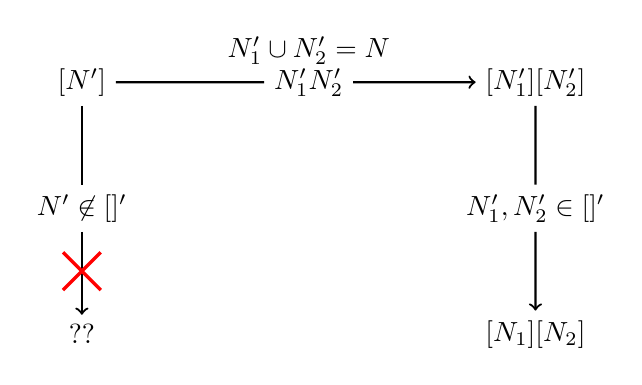
\begin{tikzpicture}[scale=0.8]
            \pgfmathsetmacro{\hs}{1.8};
            \pgfmathsetmacro{\vs}{1};
            \pgfmathsetmacro{\cross}{0.3};
            \draw (0*\hs, 4*\vs) node[](a){$\prob[N']$};
            \draw (0*\hs, 2*\vs) node[](ab){$N' \not \in \Inj[\graph]{\graph'}$};
            \draw (4*\hs, 4*\vs) node[](c){$\prob[N_1']\prob[N_2']$};
            \draw (2*\hs, 4*\vs) node[](ac){$N_1' \ancestralindep N_2'$};
            \draw (2*\hs, 4*\vs + 0.5*\vs) node[]{$N_1' \cup N_2' = N$};
            \draw (4*\hs, 2*\vs) node[](cd){$N_1', N_2' \in \Inj[\graph]{\graph'}$};
            \draw (4*\hs, 0*\vs) node[](d){$\prob[N_1]\prob[N_2]$};
            \draw (0, 0) node[](b){??};
            \draw[thick, ] (a) -- (ab);
            \draw[thick, ] (c) -- (cd);
            \draw[thick, ] (a) -- (ac);
            \draw[thick, ->] (ac) -- (c);
            \draw[thick, ->] (ab) -- (b);
            \draw[thick, ->] (cd) -- (d);
            \draw[very thick, red]
            (+ \cross, 1*\vs + \cross) -- (- \cross, 1*\vs - \cross)
            (+ \cross, 1*\vs - \cross) -- (- \cross, 1*\vs + \cross)
            ;
        \end{tikzpicture}
    \end{center}
    \begin{itemize}
        \item \textbf{Polynomial inequality} for $\graph$!
    \end{itemize}
\end{frame}

\begin{frame}
    \frametitle{Pre-injectable Sets}
    \begin{itemize}
        \item $d$-separation relations $+$ inflation $=$ polynomial inequalities over $\graph$
        \item Restrict focus to sets $N'$ that are partitioned into $N_1', N_2'$ $d$-separated by empty set $\emptyset$
        \item A \term{pre-injectable set} $N'$:
        \[ N' = {\coprod}_i N_i' \quad \forall i: N_i' \in \Inj[\graph]{\graph'} \]
        \[ \forall i, j : N_i' \ancestralindep N_j' \iff \An[\graph']{N'_i} \cap \An[\graph']{N'_j} = \emptyset \]
        \item Only need to consider \term{maximal pre-injectable sets} $\PreInj[\graph]{\graph'}$
    \end{itemize}
\end{frame}


\begin{frame}
    \frametitle{Pre-injectable Sets of Large Inflation}
    \begin{center}
        \scalebox{0.8}{\newcommand{\ift}{2.3}
\begin{tikzpicture}[scale=2]
    \begin{scope}[every node/.style=observed]
        \node (C4) at (-2, 0) {$C_4$};
        \node (C3) at ({-2 + 1/\ift}, {1/(\ift*sqrt(3))}) {$C_3$};
        \node (C2) at ({-2 + 2*1/\ift}, {2*1/(\ift*sqrt(3))}) {$C_2$};
        \node (C1) at ({-2 + 3*1/\ift}, {3*1/(\ift*sqrt(3))}) {$C_1$};
        \node (B4) at (2, 0) {$B_4$};
        \node (B3) at ({2 - 1/\ift}, {1/(\ift*sqrt(3))}) {$B_3$};
        \node (B2) at ({2 - 2*1/\ift}, {2*1/(\ift*sqrt(3))}) {$B_2$};
        \node (B1) at ({2 - 3*1/\ift}, {3*1/(\ift*sqrt(3))}) {$B_1$};
        \node (A4) at (0, {2*sqrt(3)}) {$A_4$};
        \node (A3) at (0, {2*sqrt(3) - 2/sqrt(3)*(1/\ift)}) {$A_3$};
        \node (A2) at (0, {2*sqrt(3) - 2*2/sqrt(3)*(1/\ift)}) {$A_2$};
        \node (A1) at (0, {2*sqrt(3) - 3*2/sqrt(3)*(1/\ift)}) {$A_1$};
    \end{scope}
    \begin{scope}[every node/.style=latent]
        \node (X2) at (-1, {sqrt(3)}) {$X_2$};
        \node (X1) at ({-1 + 1/\ift}, {sqrt(3) - 1/(\ift*sqrt(3))}) {$X_1$};
        \node (Y2) at (1, {sqrt(3)}) {$Y_2$};
        \node (Y1) at ({1 - 1/\ift}, {sqrt(3) - 1/(\ift*sqrt(3))}) {$Y_1$};
        \node (Z1) at (0, 0.5) {$Z_1$};
        \node (Z2) at (0, 0) {$Z_2$};
    \end{scope}
    \begin{scope}[every path/.style={draw=cause, thick}]
        \path[postaction={on each segment={mid arrow}}]
        (X2) -- (A4) (X2) -- (C4) (X2) -- (C2) (X2) -- (A3)
        (Y2) -- (A4) (Y2) -- (B4) (Y2) -- (A2) (Y2) -- (B3)
        (Z2) -- (B4) (Z2) -- (C4) (Z2) -- (B2) (Z2) -- (C3)
        (X1) -- (A1) (X1) -- (C1) (X1) -- (C3) (X1) -- (A2)
        (Y1) -- (A1) (Y1) -- (B1) (Y1) -- (A3) (Y1) -- (B2)
        (Z1) -- (B1) (Z1) -- (C1) (Z1) -- (B3) (Z1) -- (C2)
        ;
    \end{scope}
\end{tikzpicture}}
    \end{center}
    \begin{itemize}
        \item Has $12$ maximal pre-injectable sets (to follow)
    \end{itemize}
\end{frame}

\begin{frame}
    \frametitle{Large Inflation Pre-injectable Sets}
    \begin{equation*}
        \begin{gathered}
            \textbf{Maximal Pre-injectable Sets} \\
            \bc{A_1, B_1, C_1, A_4, B_4, C_4} \\
            \bc{A_1, B_2, C_3, A_4, B_3, C_2} \\
            \bc{A_2, B_3, C_1, A_3, B_2, C_4} \\
            \bc{A_2, B_4, C_3, A_3, B_1, C_2} \\
            \bc{A_1, B_3, C_4} \\
            \bc{A_1, B_4, C_2} \\
            \bc{A_2, B_1, C_4} \\
            \bc{A_2, B_2, C_2} \\
            \bc{A_3, B_3, C_3} \\
            \bc{A_3, B_4, C_1} \\
            \bc{A_4, B_1, C_3} \\
            \bc{A_4, B_2, C_1}
        \end{gathered}
        \qquad
        \begin{gathered}
            \textbf{Ancestral Independences} \\
            \bc{A_1, B_1, C_1} \ancestralindep \bc{A_4, B_4, C_4} \\
            \bc{A_1, B_2, C_3} \ancestralindep \bc{A_4, B_3, C_2} \\
            \bc{A_2, B_3, C_1} \ancestralindep \bc{A_3, B_2, C_4} \\
            \bc{A_2, B_4, C_3} \ancestralindep \bc{A_3, B_1, C_2} \\
            \bc{A_1} \ancestralindep \bc{B_3} \ancestralindep \bc{C_4} \\
            \bc{A_1} \ancestralindep \bc{B_4} \ancestralindep \bc{C_2} \\
            \bc{A_2} \ancestralindep \bc{B_1} \ancestralindep \bc{C_4} \\
            \bc{A_2} \ancestralindep \bc{B_2} \ancestralindep \bc{C_2} \\
            \bc{A_3} \ancestralindep \bc{B_3} \ancestralindep \bc{C_3} \\
            \bc{A_3} \ancestralindep \bc{B_4} \ancestralindep \bc{C_1} \\
            \bc{A_4} \ancestralindep \bc{B_1} \ancestralindep \bc{C_3} \\
            \bc{A_4} \ancestralindep \bc{B_2} \ancestralindep \bc{C_1}
        \end{gathered}
    \end{equation*}
\end{frame}

\begin{frame}
    \frametitle{Deriving Inequalities}
    \begin{itemize}
        \item Inflation facilitates turning linear, inflated inequalities into polynomial deflated ones
        \item \textbf{Question:} How to derive compatibility inequalities for $\graph'$?
        \item \textbf{Answer:} Use your favorite technique for deriving compatibility inequalities:
        \begin{itemize}
            \item Entropic inequalities
            \item Finite outcome inequalities
        \end{itemize}
        \item Here we solve the marginal problem for $\mscenario = \PreInj[\graph]{\graph'}$
        \item First some notation and formalism
    \end{itemize}
\end{frame}

\begin{frame}
    \frametitle{Outcomes and Events}
    \begin{definition}
        Each variable $v$ has finite set of \term{outcomes} $O_v$. \\
        Each set of variables $V$ has finite set of \term{events} $\Events{V}$:
        \[ \Events{V} \defined \bc{s: V \to O_V \mid \forall v \in V, s\br{v} \in O_v} \]
    \end{definition}
    \begin{definition}
        The set of events over the joint variables $\Events{\jointvar}$ are termed the \term{joint events}.
    \end{definition}
    \begin{definition}
        The set of events over the marginal contexts are the \term{marginal events}
        \[ \Events{\mscenario} \defined \coprod_{V \in \mscenario} \Events{V} \]
    \end{definition}
\end{frame}

\begin{frame}
    \frametitle{Distribution Vectors}
    \begin{definition}
        The \term{joint distribution vector} $\probvec^{\jointvar}$
        \[ \probvec^{\jointvar}_j = \prob[\jointvar][j] \quad \forall j \in \Events{\jointvar}\]
    \end{definition}
    \begin{definition}
        The \term{marginal distribution vector} $\probvec^{\mscenario}$
        \[ \probvec^{\mscenario}_m = \prob[\Dom{m}][m] \quad \forall m \in \Events{\mscenario}, \Dom{m} \in \mscenario\]
    \end{definition}
    Can now write complete marginal problem as matrix multiplication:
    \[ \forall V \in \mscenario : \prob[V] = \sum_{\jointvar \setminus V} \prob[\jointvar] \iff \probvec^{\mscenario} = M \tcdot \probvec^{\jointvar} \]
\end{frame}

\begin{frame}
    \frametitle{Incidence Matrix}
    \begin{itemize}
        \item \term{Incidence matrix} $M$ is a bit-wise matrix
        \item Row-indexed by marginal events $m \in \Events{\mscenario}$
        \item Column-indexed by joint events $j \in \Events{\jointvar}$
        \[ M_{m,j} = \begin{cases}
            1 & m = j|_{\Dom{m}} \\
            0 & \text{otherwise}
        \end{cases} \]
        \begin{gather*}
        \# \text{Columns} = \abs{\Events{\jointvar}} = \prod_{v \in \jointvar} \abs{O_{v}} \\
        \# \text{Rows} = \abs{\Events{\mscenario}} = \sum_{V \in \mscenario} \prod_{v \in V} \abs{O_{v}}
        \end{gather*}

    \end{itemize}
\end{frame}

\begin{frame}[shrink=10]
    \frametitle{Example}
    Let $\jointvar$ be $3$ binary variables $\jointvar = \bc{A,B,C}$ and $\mscenario$ be the marginal scenario $\mscenario = \bc{\bc{A,B}, \bc{B,C}, \bc{A,C}}$. The incidence matrix becomes:
    \[ M = \kbordermatrix{
        (A,B,C) \:\: = & (0,0,0) & (0,0,1) & (0,1,0) & (0,1,1) & (1,0,0) & (1,0,1) & (1,1,0) & (1,1,1) \\
        (A=0, B=0) & \kone & \kone & \kzer & \kzer & \kzer & \kzer & \kzer & \kzer \\
        (A=0, B=1) & \kzer & \kzer & \kone & \kone & \kzer & \kzer & \kzer & \kzer \\
        (A=1, B=0) & \kzer & \kzer & \kzer & \kzer & \kone & \kone & \kzer & \kzer \\
        (A=1, B=1) & \kzer & \kzer & \kzer & \kzer & \kzer & \kzer & \kone & \kone \\
        (B=0, C=0) & \kone & \kzer & \kzer & \kzer & \kone & \kzer & \kzer & \kzer \\
        (B=0, C=1) & \kzer & \kone & \kzer & \kzer & \kzer & \kone & \kzer & \kzer \\
        (B=1, C=0) & \kzer & \kzer & \kone & \kzer & \kzer & \kzer & \kone & \kzer \\
        (B=1, C=1) & \kzer & \kzer & \kzer & \kone & \kzer & \kzer & \kzer & \kone \\
        (A=0, C=0) & \kone & \kzer & \kone & \kzer & \kzer & \kzer & \kzer & \kzer \\
        (A=0, C=1) & \kzer & \kone & \kzer & \kone & \kzer & \kzer & \kzer & \kzer \\
        (A=1, C=0) & \kzer & \kzer & \kzer & \kzer & \kone & \kzer & \kone & \kzer \\
        (A=1, C=1) & \kzer & \kzer & \kzer & \kzer & \kzer & \kone & \kzer & \kone
    } \]
\end{frame}

\begin{frame}
    \frametitle{Marginal Linear Program}
    \begin{itemize}
        \item Obtain inequalities from incidence matrix $M$ and known incompatible distribution $\probvec^{\mscenario}$
    \end{itemize}
    \begin{columns}[T]
        \column{0.4\linewidth}%
            \term{Marginal LP}:%
            \begin{alignat*}{2}
                & \text{minimize:} \quad&& \emptyset \tcdot x\\
                & \text{subject to:} && x \succeq 0 \\
                & && M \tcdot x = \probvec^{\mscenario} \\
            \end{alignat*}%
        \column{0.4\linewidth}%
            \term{Dual Marginal LP}:%
            \begin{alignat*}{2}
                & \text{minimize:} \quad&& y \tcdot \probvec^{\mscenario}\\
                & \text{subject to:} && y \tcdot M \succeq 0 \\
            \end{alignat*}%
    \end{columns}
    \begin{itemize}
        \item $y$ is an \term{infeasibility certificate}:
        \[ y \tcdot M \tcdot x = y \tcdot \probvec^{\mscenario} \geq 0  \]
        \item \term{Infeasibility inequality}: $y \tcdot \probvec^{\mscenario} \geq 0$
        \item Most linear programing toolkits return certificates (\href[pdfnewwindow]{http://docs.mosek.com/8.0/pythonapi/optimizer-task-gety.html}{\textit{Mosek}}, \href[pdfnewwindow]{https://www.gurobi.com/documentation/6.5/refman/farkasdual.html}{\textit{Gurobi}}, \href[pdfnewwindow]{http://www-01.ibm.com/support/docview.wss?uid=swg21400058}{\textit{CPLEX}}, \href[pdfnewwindow]{http://cvxr.com/cvx/doc/basics.html\#dual-variables}{\textit{cvxr}}/\href[pdfnewwindow]{http://cvxopt.org/userguide/coneprog.html\#linear-cone-programs}{\textit{cvxopt}}.)
    \end{itemize}
    \note[item]{It is possible to derive non-contextuality inequalities from $M$ and a known incompatible distribution $\probvec^{\mscenario}$}
    \note[item]{Note the null objective; the minimization objective is trivially always zero}
    \note[item]{The primal value of the linear program is of no interest, all that matters is its \textit{feasibility}.}
    \note[item]{If \textit{feasible}, then there exists a vector $x$ that is a valid joint distribution vector $\probvec^{\jointvar}$.}
    \note[item]{Feasibility implies that $\probvec^{\jointvar} = x$.}
    \note[item]{Infeasibility implies contextuality}
\end{frame}

\begin{frame}
    \frametitle{Known Incompatible Distribution in The Triangle Scenario}
    \cite{Fritz_2012} provides quantum-accessible distribution incompatible with TS
    \[ \prob[ABC]\br{abc} = \Tr\bs{\netperm^\intercal \rho_{AB}\otimes\rho_{BC}\otimes\rho_{CA} \netperm M_{A,a}\otimes M_{B,b} \otimes M_{C,c}} \]
    \begin{center}
        \scalebox{1.0}{\begin{tikzpicture}[scale=1]
    \begin{scope}[every node/.style=observed]
        \node (C) at (-2, 0) {$M_C$};
        \node (B) at (2, 0) {$M_B$};
        \node (A) at (0, {2*sqrt(3)}) {$M_A$};
    \end{scope}
    \begin{scope}[every node/.style=latent]
        \node (X) at (-1, {sqrt(3)}) {$\rho_{CA}$};
        \node (Y) at (1, {sqrt(3)}) {$\rho_{AB}$};
        \node (Z) at (0, 0) {$\rho_{BC}$};
    \end{scope}
    \begin{scope}[every path/.style={draw=cause, thick}]
        \path[postaction={on each segment={mid arrow}}]
        (X) -- (A)
        (X) -- (C)
        (Y) -- (A)
        (Y) -- (B)
        (Z) -- (B)
        (Z) -- (C);
    \end{scope}
\end{tikzpicture}}
    \end{center}
\end{frame}

\begin{frame}
    \frametitle{Fritz Distribution}
    The \term{Fritz Distribution $\prob[F]$}:
    \begin{itemize}
        \item three-party $\prob[F] = \prob[ABC]$
        \item each party has $4$ outcomes
    \end{itemize}
    \begin{gather*}
    \prob[F][00\textcolor{blue}{0}] = \prob[F][11\textcolor{blue}{0}] = \prob[F][30\textcolor{blue}{1}] = \prob[F][21\textcolor{blue}{1}] = \prob[F][12\textcolor{blue}{2}] = \prob[F][03\textcolor{blue}{2}] = \prob[F][23\textcolor{blue}{3}] = \prob[F][32\textcolor{blue}{3}] = \f{1}{32}\br{2 + \sqrt{2}} \\
    \prob[F][01\textcolor{blue}{0}] = \prob[F][10\textcolor{blue}{0}] = \prob[F][31\textcolor{blue}{1}] = \prob[F][20\textcolor{blue}{1}] = \prob[F][13\textcolor{blue}{2}] = \prob[F][02\textcolor{blue}{2}] = \prob[F][22\textcolor{blue}{3}] = \prob[F][33\textcolor{blue}{3}] = \f{1}{32}\br{2 - \sqrt{2}}
    \end{gather*}
    \begin{itemize}
        \item $C$'s outcome acts as measurement ``setting'' for A, B; independent of $\rho_{AB}$
        \item Correlation coarse graining $\bc{0,1,2,3} \to \bc{\br{0,3}, \br{1,2}}$
    \end{itemize}
    \[ \ba{AB | C = 0, 1, 2} = \f{1}{\sqrt{2}} \quad \ba{AB | C = 3} = - \f{1}{\sqrt{2}} \]
    \begin{itemize}
        \item Gives CHSH violation
    \end{itemize}
    \[ \ba{AB|C=0} + \ba{AB|C=1} + \ba{AB|C=2} - \ba{AB|C=3} = 2\sqrt{2} \not \leq 2 \]
\end{frame}

\begin{frame}
    \frametitle{Quantum Implementation of Fritz Distribution}
    \begin{itemize}
        \item States:
    \end{itemize}
    \begin{gather*}
        \rho_{AB} = \ket{\Psi^+}\bra{\Psi^+} \quad \rho_{BC} = \rho_{CA} = \ket{\Phi^+}\bra{\Phi^+}
    \end{gather*}
    \begin{itemize}
        \item Maximally entangled Bell states:
    \end{itemize}
    \[ \ket{\Psi^+} = \f{1}{\sqrt{2}}\br{\ket{01} + \ket{10}} \quad \ket{\Phi^+} = \f{1}{\sqrt{2}}\br{\ket{00} + \ket{11}} \]
    \begin{itemize}
        \item Measurements:
    \end{itemize}
    \begin{gather*}
        M_{A} = \bc{\ket{0\psi_0}\bra{0\psi_0}, \ket{0\psi_{\pi}}\bra{0\psi_{\pi}}, \ket{1\psi_{-\pi/2}}\bra{1\psi_{-\pi/2}}, \ket{1\psi_{\pi/2}}\bra{1\psi_{\pi/2}}} \\
        M_{B} = \bc{\ket{\psi_{\pi/4}0}\bra{\psi_{\pi/4}0}, \ket{\psi_{5\pi/4}0}\bra{\psi_{5\pi/4}0}, \ket{\psi_{3\pi/4}1}\bra{\psi_{3\pi/4}1}, \ket{\psi_{-\pi/4}1}\bra{\psi_{-\pi/4}1}} \\
        M_{C} = \bc{\ket{00}\bra{00}, \ket{01}\bra{01}, \ket{10}\bra{10}, \ket{11}\bra{11}}
    \end{gather*}
    \begin{itemize}
        \item Shorthand: $\ket{\psi_x} = \f{1}{\sqrt{2}}\br{\ket{0} + e^{ix}\ket{1}}$
    \end{itemize}
\end{frame}

\begin{frame}
    \frametitle{Notes of Fritz Distribution}
    \begin{itemize}
        \item Proof contingent on perfect correlation between $C$ and pseudo-settings
        \item Proof not robust to noise
    \end{itemize}
    \begin{problem}[2.17 in \cite{Fritz_2012}]
        Find an example of non-classical quantum correlations in TS together with a proof of its non-classicality which does not hinge on Bell’s Theorem.
    \end{problem}
    \begin{itemize}
        \item ``...would be helpful to have inequalities...''
        \item Possible to find inequalities violated by $\prob[F]$ using the Large inflation of the TS
    \end{itemize}
\end{frame}

\begin{frame}
    \frametitle{Large Inflation Incidence}
    \begin{itemize}
        \item Joint variables are all of the observable nodes $\nodes_O' = \jointvar$
        \[ \jointvar = \bc{A_1, A_2, A_3, A_4,B_1, B_2, B_3, B_4,C_1, C_2, C_3, C_4} \]
        \item Marginal scenario is composed of pre-injectable sets $\mscenario = \PreInj[\graph]{\graph'}$
        \item Inequalities violated by Fritz distribution are inherently $4$-outcome
        \item Incidence matrix $M$ is \textbf{very large} $\sim 2.25 \textsf{Gb}$
        \begin{itemize}
            \item $\# \text{Columns} = 4^{12} = 16,777,216$
            \item $\# \text{Rows} =  4\times 4^{6} + 8 \times 4^{3} = 16,896$
            \item $\# \text{Non-zero Entries} = 201,326,592$
        \end{itemize}
    \end{itemize}
\end{frame}

\begin{frame}
    \frametitle{Triangle Scenario Inequality}

\end{frame}


\begin{frame}
    \frametitle{Causal Symmetry}
    \begin{itemize}
        \item Desirable to find compatibility inequality $I$ such that
        \[ \forall \varphi \in \Perm{A,B,C} : \varphi\bs{I} = I \]
        \item Compatibility is independent of variable labels $I, \graph \to \varphi\bs{I}, \varphi\bs{\graph}$
        \item Need $\varphi\bs{\graph} = \graph$ to find new $\varphi\bs{I}$
    \end{itemize}
    \begin{definition}
        The \term{causal symmetry group} of causal structure $\graph$:
        \[ \Aut{\graph} = \bc{\varphi \in \Perm{\nodes} \mid \varphi\bs{\graph} = \graph} \]
        Strictly speaking, one needs to preserve observable nodes:
        \[ \Aut[\nodes_O]{\graph} = \bc{\varphi \in \Aut{\graph} \mid \varphi\bs{\nodes_O} = \nodes_O} \]
    \end{definition}
    \note<1>[item]{Fritz distribution is incompatible with Triangle scenario because party $C$ plays the role of measurement settings for both $A$ and $B$}
    \note<1>[item]{In order to find quantum distributions different from $P_F$ in the Triangle Scenario, it is therefore desirable to find a proof of its incompatibility (i.e. inequality) that is symmetric under exchange of parties}
    \note<1>[item]{Surprisingly, it is possible to do so!}
    \note<1>[item]{Here is how.}
    \note<1>[item]{First, we will formally define the symmetry group in question}
    \note<1>[item]{Causal symmetry group is the group of automorphisms on causal structure}
\end{frame}

\begin{frame}
    \frametitle{Causal Symmetry and Inflation}
    \begin{itemize}
        \item Causal symmetry group for $\graph'$ is no good!
        \item Not possible to deflate inequality if it's not in terms of injectable sets
        \begin{definition}
            The \term{restricted causal symmetry group} $\Phi$ of $\graph'$:
            \[ \Phi = \Aut[\PreInj[\graph]{\graph'}]{\graph'} \]
        \end{definition}
    \end{itemize}
\end{frame}

\begin{frame}
    \frametitle{Restricted Causal Symmetry of Large Inflation}
    \begin{itemize}
        \item $\Phi$ for the large inflation is an order $48$ group with $4$ generators
    \end{itemize}
    \begin{equation*}
    \begin{aligned}[c]
    &\hspace{1mm}\gep_1 \\
    A_1 &\to A_4 \\A_2 &\to A_3 \\A_3 &\to A_2 \\A_4 &\to A_1 \\B_1 &\to B_4 \\B_2 &\to B_3 \\B_3 &\to B_2 \\B_4 &\to B_1 \\C_1 &\to C_4 \\C_2 &\to C_3 \\C_3 &\to C_2 \\C_4 &\to C_1
    \end{aligned}
    \quad
    \begin{aligned}[c]
    &\hspace{1mm}\gep_2 \\
    A_1 &\to A_1 \\A_2 &\to A_3 \\A_3 &\to A_2 \\A_4 &\to A_4 \\B_1 &\to C_1 \\B_2 &\to C_3 \\B_3 &\to C_2 \\B_4 &\to C_4 \\C_1 &\to B_1 \\C_2 &\to B_3 \\C_3 &\to B_2 \\C_4 &\to B_4
    \end{aligned}
    \quad
    \begin{aligned}[c]
    &\hspace{1mm}\gep_3 \\
    A_1 &\to C_1 \\A_2 &\to C_2 \\A_3 &\to C_3 \\A_4 &\to C_4 \\B_1 &\to A_1 \\B_2 &\to A_2 \\B_3 &\to A_3 \\B_4 &\to A_4 \\C_1 &\to B_1 \\C_2 &\to B_2 \\C_3 &\to B_3 \\C_4 &\to B_4
    \end{aligned}
    \quad
    \begin{aligned}[c]
    &\hspace{1mm}\gep_4 \\
    A_1 &\to A_1 \\A_2 &\to A_2 \\A_3 &\to A_3 \\A_4 &\to A_4 \\B_1 &\to B_2 \\B_2 &\to B_1 \\B_3 &\to B_4 \\B_4 &\to B_3 \\C_1 &\to C_3 \\C_2 &\to C_4 \\C_3 &\to C_1 \\C_4 &\to C_2
    \end{aligned}
    \end{equation*}
\end{frame}

\begin{frame}
    \frametitle{Symmetric Incidence}
    \begin{itemize}
        \item Group orbits through repeated action of $\varphi \in \Phi$ on $m \in \Events{\mscenario}$ and $j \in \Events{\jointvar}$
    \end{itemize}
    \begin{align*}
        \Phi\bs{m} &\defined \bc{\varphi\bs{m} \mid \varphi \in \Phi} \\
        \Phi\bs{j} &\defined \bc{\varphi\bs{j} \mid \varphi \in \Phi}
    \end{align*}
    \begin{itemize}
        \item Construct \term{symmetric incidence matrix} $\Phi\bs{M}$
    \end{itemize}
    \[ \Phi\bs{M}_{\Phi\bs{m}, \Phi\bs{j}} = \sum_{m' \in \Phi\bs{m}}\sum_{j' \in \Phi\bs{j}} M_{m',j'} \]
    \[ \Phi\bs{M} = \La_{\Phi\bs{\Events{\mscenario}}}\tcdot M \tcdot \La_{\Phi\bs{\Events{\jointvar}}} \]
    \begin{itemize}
        \item $\Phi\bs{M}$ not a bit-wise matrix like $M$
        \item For large inflation $M$ is $16,896 \times 16,777,216$
        \item For large inflation $\Phi\bs{M}$ is $450 \times 358,120$ % 3566922 entries
    \end{itemize}
\end{frame}

\begin{frame}[shrink=60]
    \frametitle{Party Symmetric Inequality}
    \begin{gather*}
	2[P(001)P(333)]_{3} + 2[P(010)P(323)]_{3} + 6[P(000)P(323)]_{3} + 6[P(000)P(333)]_{1}
\end{gather*}
\[\leq\]
\begin{gather*}
	12[P(031)P(302)]_{6} + 12[P(033)P(303)]_{6} + 12[P(103)P(130)]_{6} + 12[P(203)P(230)]_{6} + 12[P(203)P(330)]_{6} + 2[P(001)P(320)]_{6} + 2[P(002)P(221)]_{3} + 2[P(003)P(211)]_{6}+ \\
	2[P(003)P(331)]_{3} + 2[P(011)P(211)]_{3} + 2[P(012)P(322)]_{6} + 2[P(013)P(313)]_{6} + 2[P(013)P(332)]_{6} + 2[P(020)P(111)]_{3} + 2[P(020)P(211)]_{6} + 2[P(021)P(212)]_{6}+ \\
	2[P(022)P(211)]_{3} + 2[P(022)P(212)]_{6} + 2[P(022)P(322)]_{3} + 2[P(023)P(232)]_{6} + 2[P(030)P(212)]_{3} + 2[P(031)P(231)]_{6} + 2[P(032)P(331)]_{6} + 2[P(033)P(333)]_{3}+ \\
	2[P(101)P(131)]_{3} + 2[P(101)P(132)]_{6} + 2[P(102)P(131)]_{6} + 2[P(102)P(132)]_{6} + 2[P(102)P(133)]_{6} + 2[P(110)P(133)]_{6} + 2[P(110)P(212)]_{6} + 2[P(110)P(222)]_{3}+ \\
	2[P(110)P(223)]_{3} + 2[P(112)P(331)]_{3} + 2[P(120)P(122)]_{6} + 2[P(121)P(201)]_{6} + 2[P(122)P(200)]_{3} + 2[P(122)P(202)]_{6} + 2[P(122)P(210)]_{6} + 2[P(122)P(300)]_{3}+ \\
	2[P(130)P(232)]_{6} + 2[P(130)P(233)]_{6} + 2[P(131)P(201)]_{6} + 2[P(131)P(202)]_{3} + 2[P(131)P(313)]_{3} + 2[P(133)P(200)]_{3} + 2[P(133)P(201)]_{6} + 2[P(133)P(211)]_{3}+ \\
	2[P(133)P(212)]_{6} + 2[P(133)P(300)]_{3} + 2[P(202)P(231)]_{6} + 2[P(210)P(222)]_{6} + 2[P(220)P(222)]_{3} + 2[P(220)P(313)]_{6} + 2[P(221)P(313)]_{6} + 2[P(222)P(331)]_{3}+ \\
	2[P(223)P(331)]_{3} + 2[P(230)P(312)]_{6} + 2[P(231)P(313)]_{6} + 2[P(232)P(320)]_{6} + 2[P(302)P(322)]_{6} + 2[P(320)P(323)]_{6} + 2[P(330)P(332)]_{3} + 3[P(000)P(003)]_{3}+ \\
	3[P(010)P(301)]_{6} + 4[P(001)P(131)]_{6} + 4[P(002)P(020)]_{6} + 4[P(002)P(133)]_{6} + 4[P(002)P(323)]_{6} + 4[P(010)P(123)]_{6} + 4[P(013)P(212)]_{6} + 4[P(013)P(312)]_{6}+ \\
	4[P(023)P(221)]_{6} + 4[P(023)P(222)]_{6} + 4[P(023)P(322)]_{6} + 4[P(031)P(211)]_{6} + 4[P(032)P(321)]_{6} + 4[P(100)P(123)]_{6} + 4[P(100)P(232)]_{6} + 4[P(100)P(313)]_{6}+ \\
	4[P(112)P(310)]_{6} + 4[P(122)P(203)]_{6} + 4[P(122)P(302)]_{6} + 4[P(130)P(222)]_{6} + 4[P(130)P(223)]_{6} + 4[P(222)P(310)]_{6} + 4[P(223)P(320)]_{6} + 4[P(231)P(301)]_{6}+ \\
	4[P(312)P(330)]_{6} + 6[P(001)P(031)]_{6} + 6[P(001)P(033)]_{6} + 6[P(002)P(300)]_{6} + 6[P(002)P(330)]_{3} + 6[P(003)P(032)]_{6} + 6[P(003)P(131)]_{6} + 6[P(003)P(132)]_{6}+ \\
	6[P(011)P(300)]_{3} + 6[P(011)P(320)]_{6} + 6[P(012)P(200)]_{6} + 6[P(012)P(301)]_{6} + 6[P(013)P(030)]_{6} + 6[P(013)P(110)]_{6} + 6[P(013)P(120)]_{6} + 6[P(013)P(303)]_{6}+ \\
	6[P(020)P(102)]_{6} + 6[P(020)P(103)]_{6} + 6[P(020)P(123)]_{6} + 6[P(020)P(202)]_{3} + 6[P(020)P(203)]_{6} + 6[P(020)P(311)]_{6} + 6[P(020)P(322)]_{6} + 6[P(020)P(330)]_{6}+ \\
	6[P(022)P(303)]_{6} + 6[P(030)P(033)]_{6} + 6[P(030)P(101)]_{3} + 6[P(030)P(133)]_{6} + 6[P(030)P(202)]_{3} + 6[P(030)P(303)]_{3} + 6[P(030)P(332)]_{6} + 6[P(031)P(203)]_{6}+ \\
	6[P(032)P(310)]_{6} + 6[P(033)P(101)]_{6} + 6[P(033)P(130)]_{6} + 6[P(033)P(200)]_{3} + 6[P(033)P(212)]_{6} + 6[P(033)P(220)]_{6} + 6[P(033)P(222)]_{3} + 6[P(033)P(230)]_{6}+ \\
	6[P(033)P(322)]_{3} + 6[P(100)P(203)]_{6} + 6[P(101)P(130)]_{6} + 6[P(103)P(310)]_{6} + 6[P(113)P(130)]_{6} + 6[P(113)P(230)]_{6} + 6[P(113)P(330)]_{3} + 6[P(122)P(330)]_{6}+ \\
	6[P(130)P(313)]_{6} + 6[P(132)P(303)]_{6} + 6[P(133)P(303)]_{6} + 6[P(133)P(320)]_{6} + 6[P(200)P(203)]_{6} + 6[P(201)P(230)]_{6} + 6[P(203)P(231)]_{6} + 6[P(223)P(300)]_{6}+ \\
	8[P(003)P(320)]_{6} + 8[P(032)P(300)]_{6}
\end{gather*}
\end{frame}


\begin{frame}
    \frametitle{Parameterizing Quantum Distributions}
    For our purposes, we need to parameterize the space of quantum-accessible distributions that are \textit{realized} on the Triangle Scenario
    \[ \prob[ABC]\br{abc} = \Tr\bs{\netperm^\intercal \rho_{AB}\otimes\rho_{BC}\otimes\rho_{CA} \netperm M_{A,a}\otimes M_{B,b} \otimes M_{C,c}} \]
    \begin{center}
        \scalebox{1.0}{\begin{tikzpicture}[scale=1]
    \begin{scope}[every node/.style=observed]
        \node (C) at (-2, 0) {$M_C$};
        \node (B) at (2, 0) {$M_B$};
        \node (A) at (0, {2*sqrt(3)}) {$M_A$};
    \end{scope}
    \begin{scope}[every node/.style=latent]
        \node (X) at (-1, {sqrt(3)}) {$\rho_{CA}$};
        \node (Y) at (1, {sqrt(3)}) {$\rho_{AB}$};
        \node (Z) at (0, 0) {$\rho_{BC}$};
    \end{scope}
    \begin{scope}[every path/.style={draw=cause, thick}]
        \path[postaction={on each segment={mid arrow}}]
        (X) -- (A)
        (X) -- (C)
        (Y) -- (A)
        (Y) -- (B)
        (Z) -- (B)
        (Z) -- (C);
    \end{scope}
\end{tikzpicture}}
    \end{center}
\end{frame}

\begin{frame}
    \frametitle{Numerical Optimization}
    \begin{itemize}
        \item Attempt to find new non-classical distributions
        \item Objective function $f\br{\la} \in \R$
        \begin{enumerate}
            \item Real-valued parameters $\la = \br{\la_0, \ldots, \la_n}$
            \item Quantum states/measurements $\rho_{AB}, \rho_{BC}, \rho_{CA}, M_{A}, M_{B}, M_{C}$
            \item Distribution $\prob[ABC]$
            \item Plug into inequality $I$ in homogeneous form $I\br{\prob[ABC]} \geq 0$
            \item Output is objective value $I\br{\prob[ABC]}$
        \end{enumerate}
        \item Numerical minimization of $f\br{\la}$
        \[ f(\la_{(k+1)}) = \la_{(k)} - \ga_{(k)} \del f(\la_{(k)})  \]
        \item Non-convex, non-linear, smooth/continuous
        \item Gradient Descent, BFGS Method, Nelder-Mead simplex method
        \item Stochastic methods: simulated annealing, basin-hopping
    \end{itemize}
\end{frame}

\begin{frame}
    \frametitle{Parameterizing Unitary Group}
    \begin{itemize}
        \item Spengler, Huber and Heismayr \cite{Spengler_2010_Unitary} demonstrate a parameterization of $\s{U}\br{d}$ where the parameters are organized in a $d \times d$-matrix of real values $\la_{n,m}$
        \[ U = \bs{\prod_{m=1}^{d-1} \br{\prod_{n=m+1}^{d} R_{m,n} RP_{n,m}}} \tcdot \bs{\prod_{l=1}^{d} GP_{l}} \]
        \item Global Phase Terms: $GP_{l} = \exp\br{iP_l \lambda_{l,l}}$
        \item Relative Phase Terms: $RP_{n,m} = \exp\br{i P_n \lambda_{n,m}}$
        \item Rotation Terms: $R_{m,n} = \exp\br{i \si_{m,n} \lambda_{m,n}}$
        \item Projection Operators: $P_l = \ket{l}\bra{l}$
        \item Anti-symmetric $\si$-matrices: $\si_{m,n} = - i\ket{m}\bra{n} + i \ket{n}\bra{m}$
        \item Parameters $\la_{n,m} \in \bs{0, 2\pi}$
    \end{itemize}
\end{frame}

\begin{frame}
    \frametitle{Parameterizing Unitary Group Cont'd}
    \begin{itemize}
        \item Each parameter $\la_{n,m}$ has physical interpretation
        \item Degeneracies are easily eliminated such as global phase
        \[ \forall l = 1, \ldots, d : \la_{l,l} = 0 \implies GP_{l} = \ident \]
        \item Parameterize $U \in \s{U}\br{d}$ up to global phase denoted $\ti{U} \in \s{U}\br{d}$
        \item Computationally efficient
        \begin{alignat*}{2}
            GP_l &= \ident &&+ P_l \br{e^{i\la_{l,l}} - 1} \\
            RP_{n,m} &= \ident &&+ P_n \br{e^{i\la_{n,m}} - 1} \\
            R_{m,n} &= \ident &&+ \br{\ket{m}\bra{m} + \ket{n}\bra{n}} \br{\cos\lambda_{n,m} - 1} \\
            & &&+ \br{\ket{m}\bra{n} - \ket{n}\bra{m}} \sin\lambda_{n,m} \\
        \end{alignat*}
    \end{itemize}
\end{frame}

\begin{frame}
    \frametitle{Parameterizing States}
    \begin{itemize}
        \item Each latent resource $\rho \in \br{\rho_{AB}, \rho_{BC}, \rho_{CA}}$ modeled as bipartite qubit state acting on $\Hilb^{d/2} \otimes \Hilb^{d/2}$
        \item $d \times d$ positive semi-definite (PSD) hermitian matrices with unitary trace
        \item \term{Cholesky Parametrization} allows one to write any hermitian PSD as $\rho = T^{\dagger} T$
        \item For $d = 4$:
        \[ T = \begin{bmatrix}\la_{1}&0&0&0\\\la_{2} + i \la_{3}&\la_{4}&0&0\\\la_{5} + i \la_{6}&\la_{7} + i \la_{8}&\la_{9}&0\\\la_{10} + i \la_{11}&\la_{12} + i \la_{13}&\la_{14} + i \la_{15}&\la_{16}\end{bmatrix} \]
        \item $d^2$ real-valued parameters
        \item Normalized $\rho = {T^{\dagger}T}/{\Tr\br{T^{\dagger} T}}$ adds degeneracy
    \end{itemize}
\end{frame}

\begin{frame}
    \frametitle{Parameterizing States Cont'd}
    \begin{itemize}
        \item \term{SHH parameterization} \cite{Spengler_2010_Unitary} exploits spectral decomposition; for rank $k \leq d$ density matrix
        \[ \rho = \sum_{i=1}^{k} p_i \ket{\psi_i} \bra{\psi_i} \qquad p_i \geq 0, \sum_i p_i = 1 \]
        \item Orthonormal $k$-element sub-basis $\bc{\ket{\psi_i}}$ of $\Hilb^d$ can be transformed into computational basis $\bc{\ket{i}}$ by unitary $U \in \s{U}\br{d}$ such that $\ket{\psi_i} = U \ket{i}$
        \item Freedom to choice $k$
        \item Parameterize $\rho$ through $\bc{p_i}$ and $\ti{U}_{k}$
        \[ \ti{U}_{k} = \prod_{m=1}^{k} \br{\prod_{n={m+1}}^{d} R_{m,n} RP_{n,m}} \]
        \item real-value parameters $d^2 - \br{d-k}^2 - k$ for $\ti{U}_{k}$, $k-1$ for $\bc{p_i}$ (no degeneracy)
    \end{itemize}
\end{frame}

\begin{frame}
    \frametitle{Parameterizing POVMs}
    \begin{itemize}
        \item Each party $\br{A, B, C}$ is assigned a \term{projective-operator valued measure (POVM)} $\br{M_A, M_B, M_C}$
        \[ \forall \ket{\psi} \in \Hilb^d : \bra{\psi} M_\chi \ket{\psi} \geq 0 \quad M_\chi = M_\chi^{\dagger} \]
        \item $n$-outcome measurement
        \[ M_\chi = \bc{M_{\chi, 1}, \ldots, M_{\chi, n}} \quad \sum_{i=1}^{n} M_{\chi, i} = \ident \]
        \item For $n = 2$ outcomes, a parameterization exists by constraining the eigenvalues of $M_{\chi, i}$; for $n > 2$ not aware of anything
        \item Warrants consideration of \term{projective-valued measures (PVMs)} (for $n = d$ this is without loss of generality)
    \end{itemize}
    \note<1>[item]{Naimark's Dilation Theorem}
\end{frame}

\begin{frame}
    \frametitle{Parameterizing PVMs}
    \begin{itemize}
        \item Each party $\br{A, B, C}$ is assigned $n$-outcome $\br{M_A, M_B, M_C}$ such that,
        \[ M_{\chi,i}M_{\chi,j} = \de_{ij} M_{\chi, i} \quad M_{\chi, i} = \ket{m_{\chi,i}}\bra{m_{\chi,i}} \]
        \item Inspired by \cite{Pal_2010}, parameterizing PVMs means parameterizing a $n$-element sub-basis $\bc{\ket{m_{\chi,i}}}$
        \item Use unitary transformation again
        \[ \bc{\ket{m_{\chi,1}}, \ldots, \ket{m_{\chi,n}}} = \bc{U \ket{1}, \ldots, U \ket{n}} \]
        \item Global phase and remaining basis irrelevant: $\ti{U}_{n}$ requires $n(2d - n - 1)$ real-valued parameters\
        \item PVMs are computationally more efficient
    \end{itemize}
    \[ \prob[ABC]\br{abc} = \bra{m_{A,a}m_{B,b}m_{C,c}}{\netperm^\intercal \rho_{AB}\otimes\rho_{BC}\otimes\rho_{CA} \netperm}\ket{m_{A,a}m_{B,b}m_{C,c}} \]
\end{frame}

\begin{frame}
    \frametitle{Network Permutation Matrix}
    \begin{columns}
        \column{0.6\linewidth}
        \begin{itemize}
            \item States and measurements in the Triangle Scenario are not aligned
            \item Without $\netperm$, $\prob[ABC]$ would be separable
            \item Required to align $B$'s measurement over $\Tr_{A,C}\br{\rho_{AB} \otimes \rho_{BC}}$
            \item $\netperm$ is a $2^6 \times 2^6$ matrix
            \item Shifts one qubit to the left
        \end{itemize}
        \column{0.4\linewidth}
            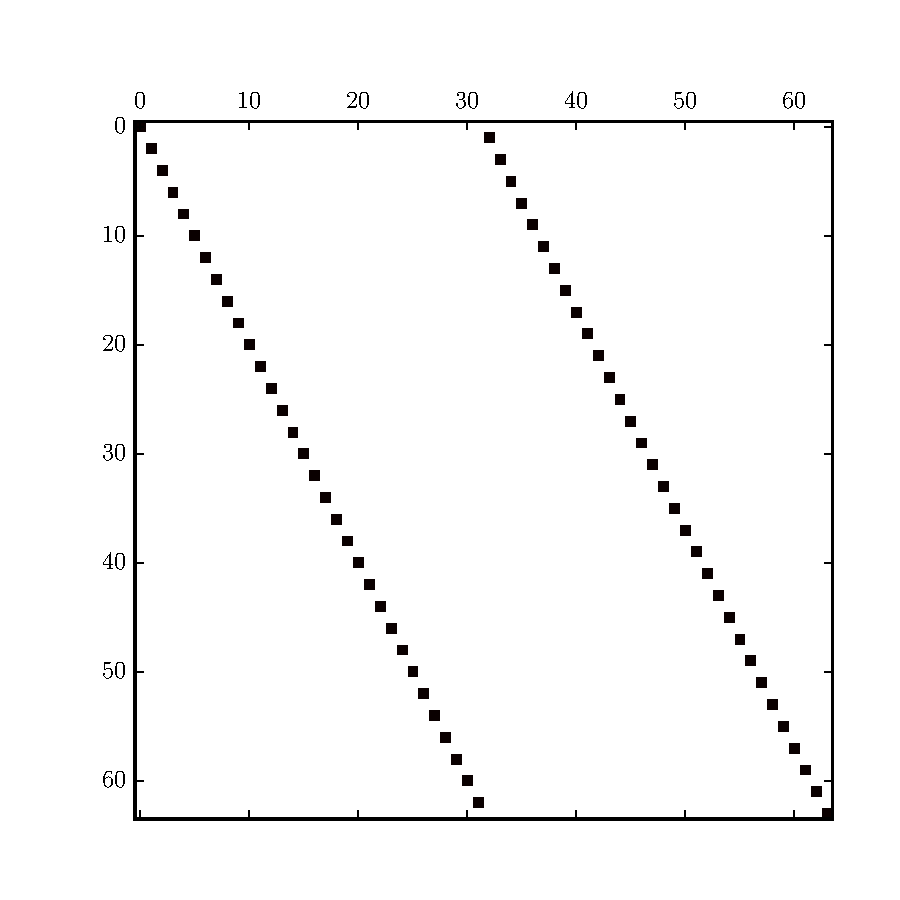
\includegraphics[trim={1.0cm 1.2cm 1.0cm 1cm},clip,width=1.0\textwidth]{../../figures/perm_mtrx.pdf}
    \end{columns}
    \[ \netperm \defined \sum_{\ket{q_i} \in \bc{\ket{0}, \ket{1}}}\ket{q_2q_3q_4q_5q_6q_1}\bra{q_1q_2q_3q_4q_5q_6} \]
\end{frame}

\begin{frame}
    \frametitle{Results}
    \begin{itemize}
        \item Full rank $\rho, M$ gives $81$ free parameters
        \[ \abs{\la} = 3 \cdot (12 + 3) + 3 \cdot 12 = 81 \]
        \item Parameterization of quantum distributions still degenerate
        \item Noisy seed (Gaussian noise):
        \[ \la_{(0)} = \la_{(F)} + \de \la \qquad \de \la_{i} \sim \s{N}\br{\mu = 0, \si^2 = (2\pi10^{\chi})^2} \]
        \item Uniform seed:
        \[ \la_{(0), i} \sim \s{U}\br{[0, 2\pi]} \]
    \end{itemize}

\end{frame}

\begin{frame}
    \frametitle{Fritz Local Minima}
    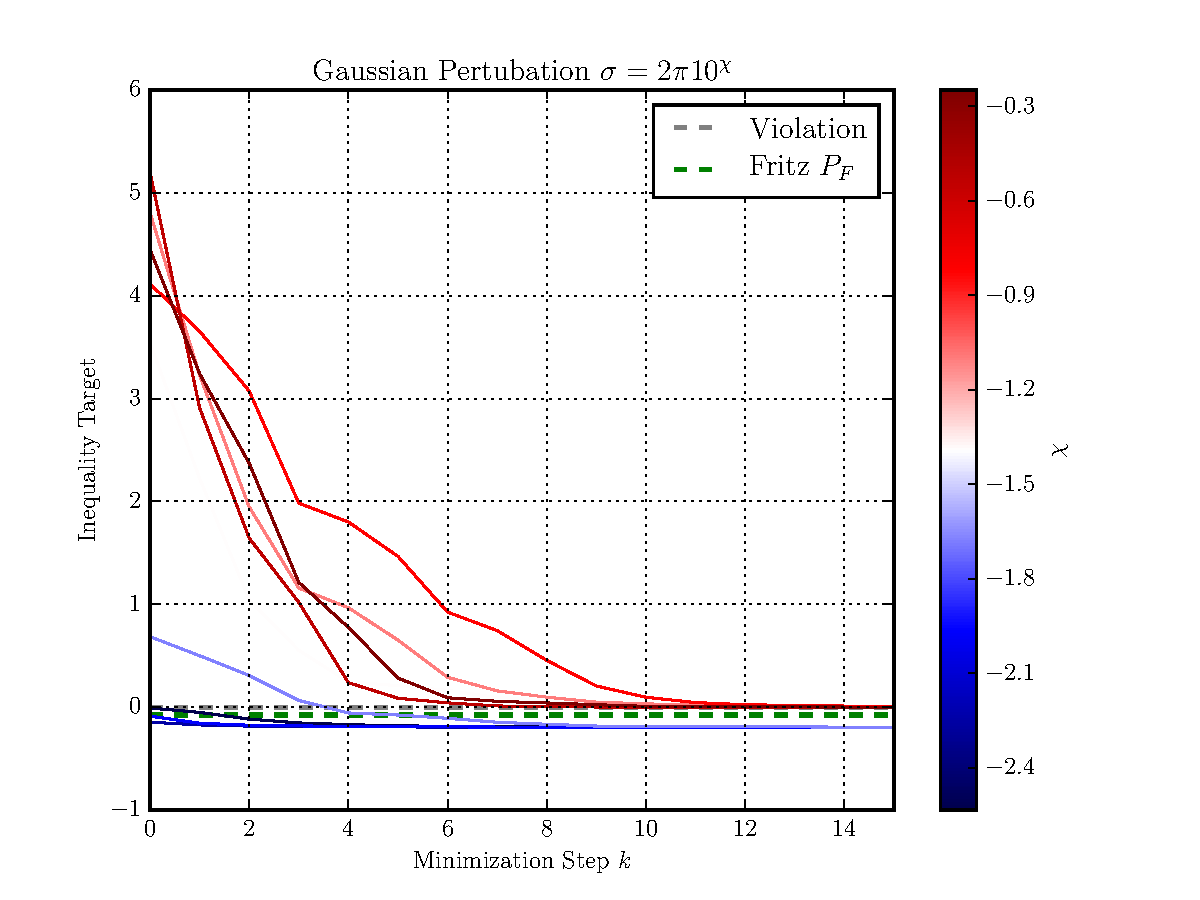
\includegraphics[width=\linewidth]{../../figures/optimizations/Gaussian_Perturbation_Fritz_Color_Default.pdf}
\end{frame}

\begin{frame}
    \frametitle{Fritz Local Minima Zoomed}
    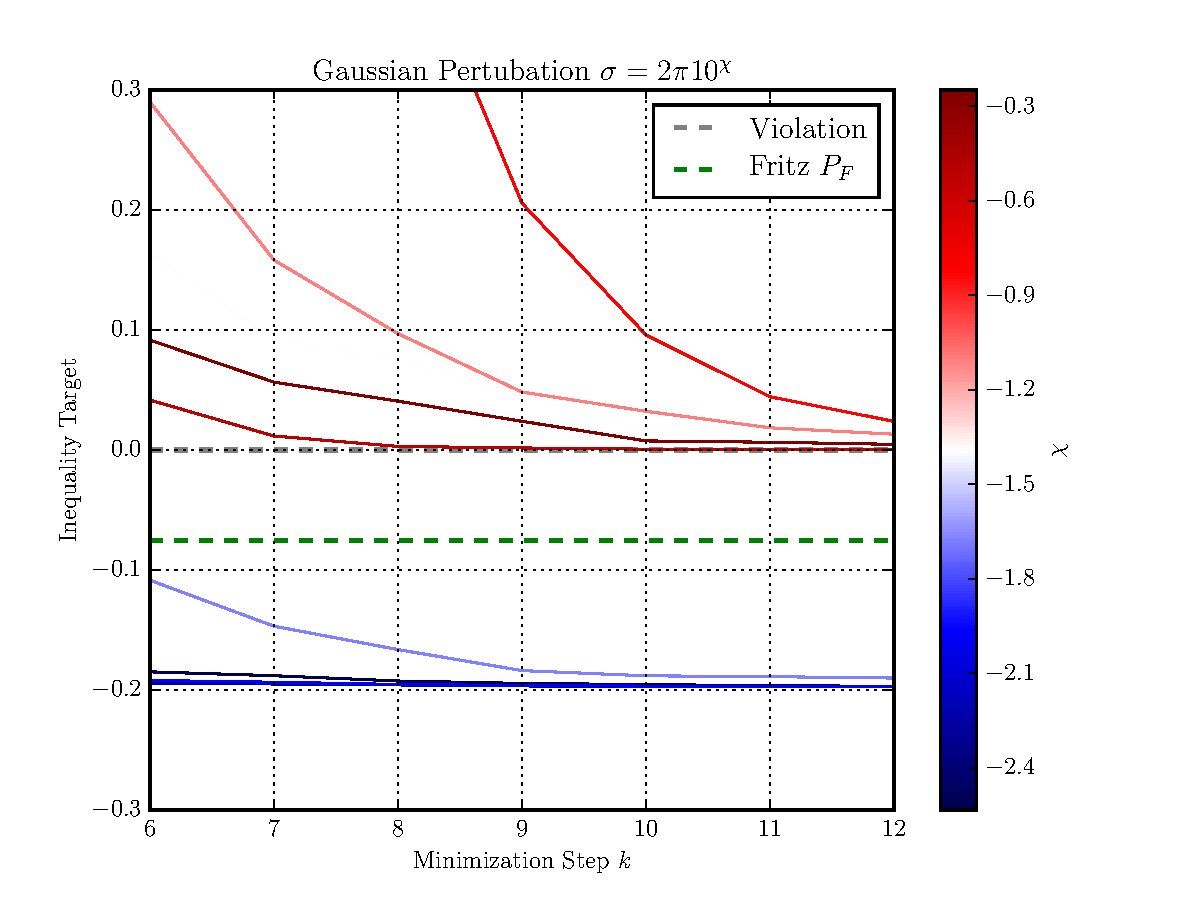
\includegraphics[width=\linewidth]{../../figures/optimizations/Gaussian_Perturbation_Fritz_Color_Zoomed.pdf}
\end{frame}

\begin{frame}
    \frametitle{Max Entangled vs. Max Violating (???) [Optional]}
    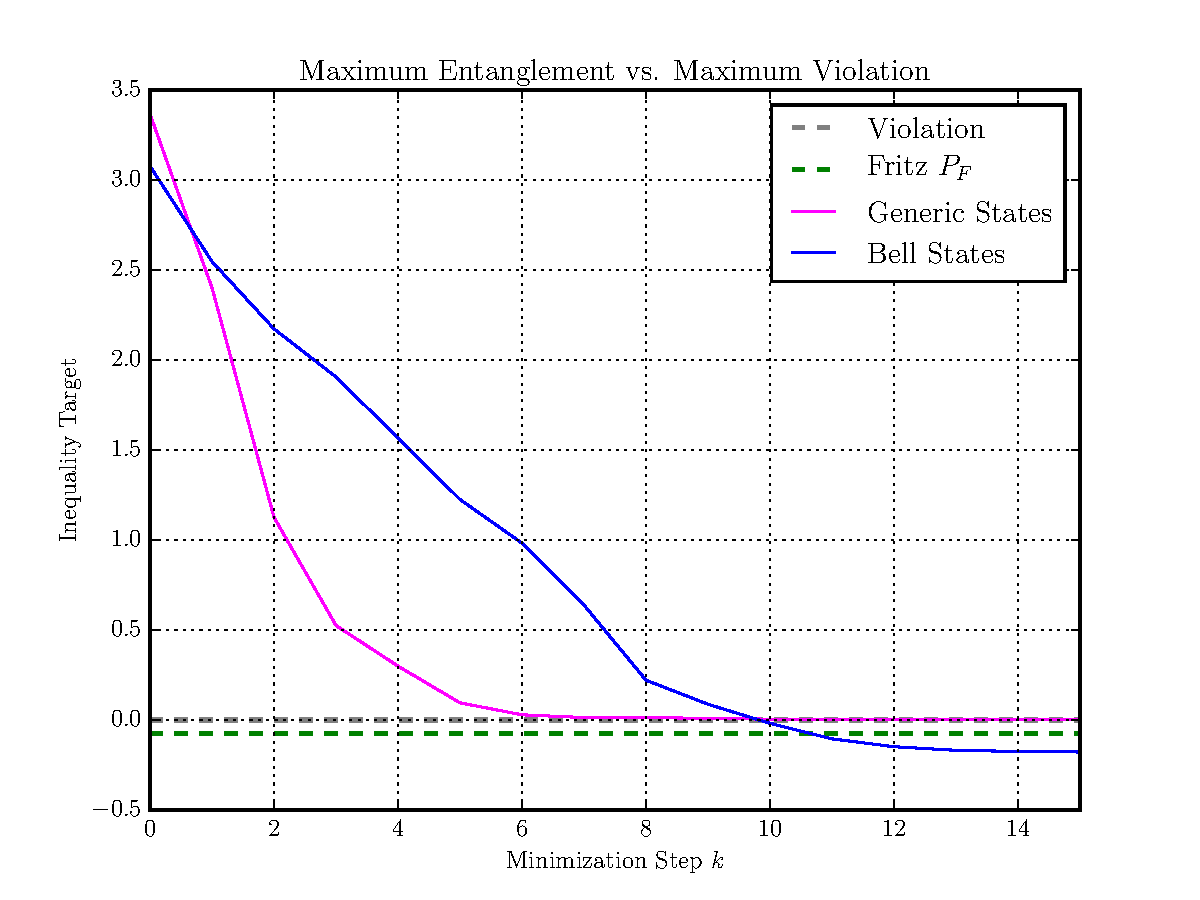
\includegraphics[width=\linewidth]{../../figures/optimizations/Max_Entanglement_vs_Max_Violation_random_seed.pdf}
\end{frame}

\begin{frame}
    \frametitle{Max Entangled vs. Max Violating (???) [Optional]}
    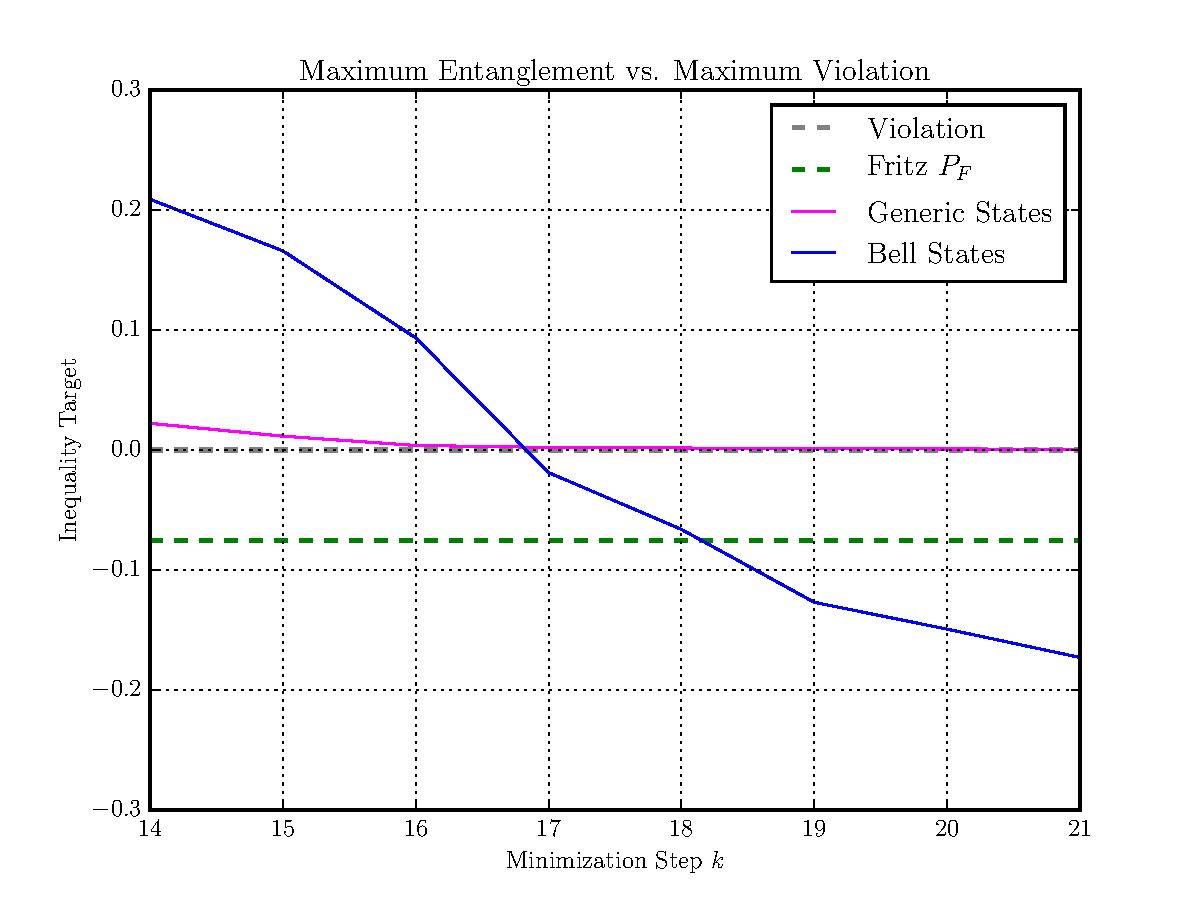
\includegraphics[width=\linewidth]{../../figures/optimizations/Max_Entanglement_vs_Max_Violation_random_seed_Zoomed.pdf}
\end{frame}

\begin{frame}
    \frametitle{Max Entangled vs. Max Violating} % $\chi = -2$
    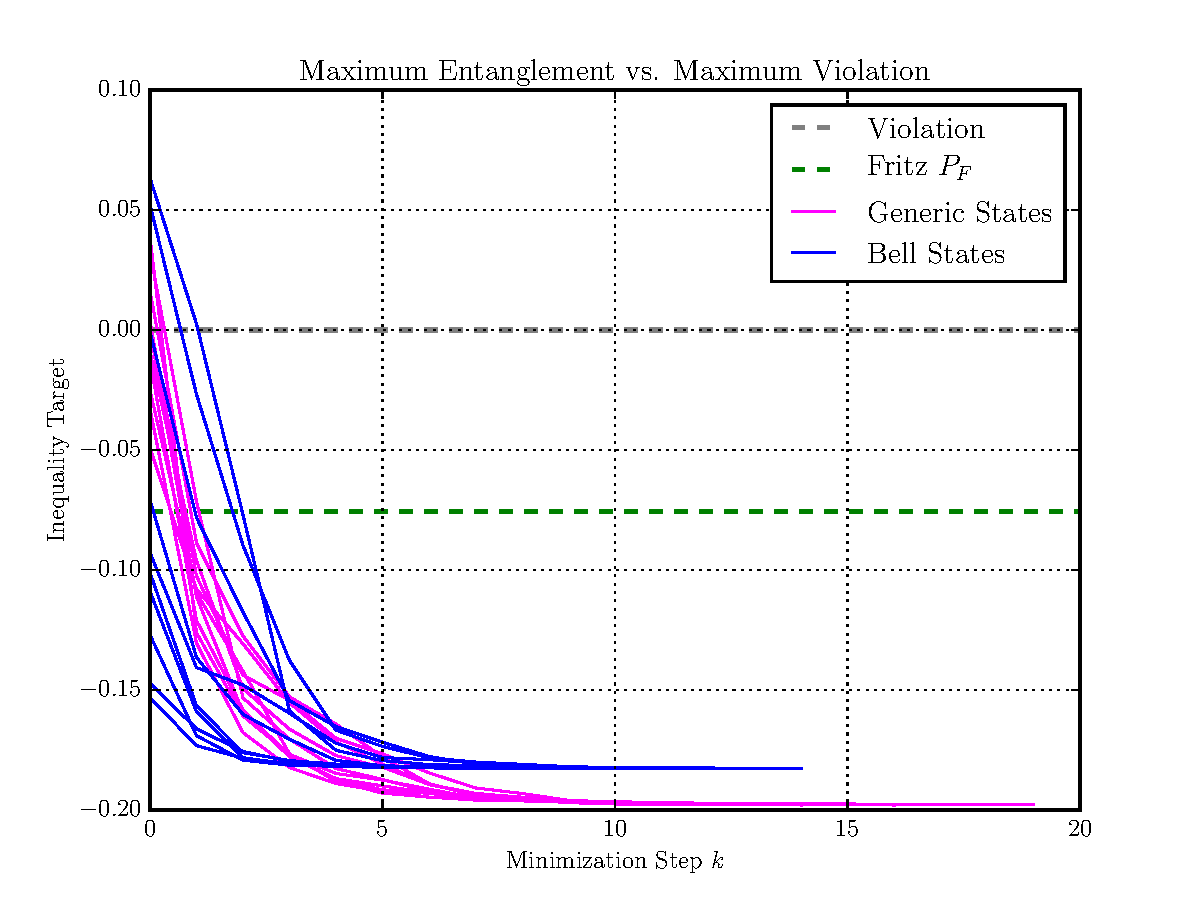
\includegraphics[width=\linewidth]{../../figures/optimizations/Max_Entanglement_vs_Max_Violation_fritz_seed.pdf}
\end{frame}

\begin{frame}
    \frametitle{Maximally Violating Distributions}
    \begin{itemize}
        \item Able to out-perform violation provided by Fritz distribution
        \item Maximally-violating states are not maximally-entangled; similar to detection loop-hole example of \cite{Methot_2006}
        \item Violation very sensitive to the initial parameters $\la_{(0)}$
        \item Both symmetric and asymmetric inequalities exhibit same qualitative features
    \end{itemize}
\end{frame}

\begin{frame}
    \frametitle{Conclusions}
    \begin{itemize}
        \item New causal compatibility inequalities have been found for the TS
        \item Inflation technique capable of producing inequalities with quantum/classical witnesses
        \item Proof of non-classicality is robust to noise
        \item Fritz witness-able by party symmetric inequalities
        \item Maximally violating distributions are different than Fritz but also similar
        \item Further research is necessary
    \end{itemize}
\end{frame}

\begin{frame}
    \frametitle{Post-doc Opportunities At Perimeter}
\end{frame}

\end{document}